\section{Related}

\subsection{Mixture of Experts}

From a machine learning perspective, we can view this architecture as an instance of the mixture of experts architecture.
In this case, the Mealy machine acts as the \textit{Gating Network} in Fig.~\ref{fig:MOE}.
By using an explicit structure for the gating networks (as opposed to another neural network), we enable a level of legibility over the entire system.

\begin{figure}[h]  
\centering 
    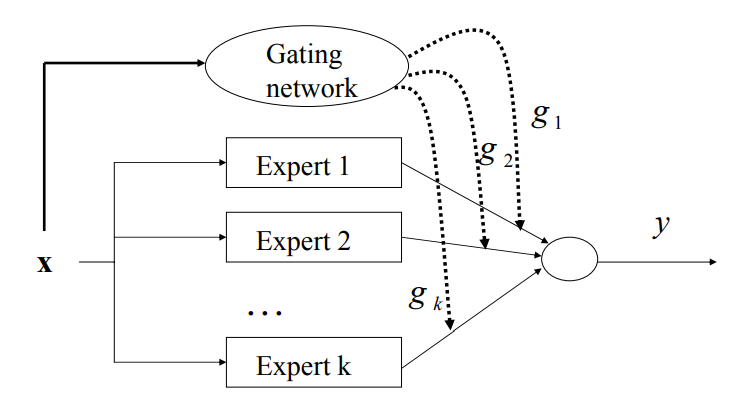
\includegraphics[width=\linewidth]{MOE.png}
    \caption{No interaction} \label{fig:M1}  
\end{figure} 

\begin{figure}[h!]  
\centering 
  \newcommand{\arrow}[3]{
  \node[anchor=west,inner sep=0pt] at #1 (#2) {
    \begin{tikzpicture}[scale=0.8,inner sep=2pt]
      \node[arrow] (A) at (-3,0) {#3};      
      \fill[green!10] (A.south east) -- (A.south west) -- 
      (A.north west) -- (A.north east) 
      -- ($ (A.east) + (0.2,0) $) -- cycle;
      \node[arrow] (A) at (-3,0) {#3};      
      \draw (A.south east) -- (A.south west) -- 
      (A.north west) -- (A.north east) -- 
      ($ (A.east) + (0.2,0) $) -- cycle;
    \end{tikzpicture}
  };
}

\sbox0{
  \begin{tikzpicture}[circuit logic US,line width=0.4,scale=0.45,remember picture]
    \tikzset{
      and/.style={and gate, inputs={nn}, point right,blue!80!black!50!white,fill},
      or/.style={or gate, inputs={nn}, point right,blue!70,fill},
      not/.style={not gate, point right, scale=0.5,black!50!blue, fill},
      sec/.style={fill, circle,inner sep=0.7pt},
    }

    \draw[fill=yellow!10,rounded corners=3,fill,drop shadow,thin] (-2,-5.9) rectangle (7.8,2);

    \node at (-2,-2.6) (pause) {}; 
    \node at (-2,1.4) (cfg) {}; 
    \node at (-2,0.7) (play) {}; 
    \node at (-2,-1.3) (resume) {};
    \node at (-2,-5.1) (leave) {};  
    \node at (-2,-5.3) (music) {}; 

    \node at (5.7,-5.9) (out1) {};
    \node at (6.5,-5.9) (out2) {};
    \node at (7.3,-5.9) (out3) {};

    \node at (7.7,0.9) (out4) {};
    \node at (7.7,1.4) (out5) {};

    \node[and] at (0.05,0.6) (a1) {};
    \node[or] at (0,-1.4) (o1) {};
    \node[or] at (0,-2.2) (o2) {};
    \node[or] at (0,-3) (o3) {};
    \node[not] at (1.1,-3) (n1) {};
    \node[not] at (1.1,-2.2) (n2) {};
    \node[not] at (1.1,0.2) (n3) {};
    \node[and] at (2.3,-1) (a2) {};
    \node[or] at (3.6,-0.5) (o4) {};
    \node[and] at (2.3,-3.7) (a3) {};
    \node[and] at (0.05,-5.2) (a4) {};
    \node[and] at (2.3,-4.5) (a5) {};
    \node[or] at (3.6,-4.1) (o5) {};
    \node[not] at (1.1,-5.2) (n4) {};
    \node[and] at (3.7,-3.1) (a6) {};
    \node[and] at (5.3,-1.8) (a7) {};
    \node[or] at (6.6,0.1) (o6) {};
    \node[or] at (5.2,0.9) (o7) {};
    \node[not] at (6.6,0.9) (n5) {};

    \draw (o1.output) ++ (right:0.2) node[sec] {} |- (n3.input);
    \draw (o1.output) -- ++ (right:0.2) |- (a3.input 1);
    \draw (o2.output) -- (n2.input);
    \draw (o3.output) -- (n1.input);
    \draw (n2.output) -- ++ (right:0.2) |- (a2.input 2);
    \draw (a2.output) -- ++ (right:0.2) |- (o4.input 2);
    \draw (a1.output) -| ($ (a2.output) + (0.2,1) $) |- (o4.input 1);
    \draw (a4.output)  ++ (right:0.25) node[sec] {} |- (a5.input 2);
    \draw (a4.output) -- (n4.input);
    \draw (a3.output) -- ++ (right:0.2) |- (o5.input 1);
    \draw (a5.output) ++ (right:0.2) |- (o5.input 2);
    \draw (a5.output) -- ++ (right:0.2) node[sec] {} |- ($ (a6.output) + (0.2,-1.7) $) |- (o7.input 2);
    \draw (n1.output) -- (a6.input 1);
    \draw (n3.output) ++ (right:0.8) node[sec] {} |- (o7.input 1);
    \draw (n3.output) -- (o6.input 1);
    \draw (n4.output) -- ++ (right:0.2) |- (a6.input 2);
    \draw (a6.output) -- ++ (right:0.5) node (A) {} |- (a7.input 2);
    \draw (a7.output) -- ++ (right:0.2) |- (o6.input 2);
    \draw (o7.output) -- (n5.input);

    \draw (o5.output) -| (out1.center);
    \draw (o4.output) -- ++ (right:2.4) |- (out2.center);
    \draw (o6.output) -- ++ (right:0.2) |- (out3.center);
    \draw (n5.output) -- (out4.center);
    \draw (o7.output) ++ (right:0.2) node[sec] {} |- (out5.center);

    \draw (pause.center) -- ++ (right:0.5) |- (o2.input 1);
    \draw (pause.center) ++ (right:0.5) node[sec] (T) {} |- node[sec] {} (o3.input 2);
    \draw (T.center |- o3.input 2) |- (a3.input 2);

    \draw (cfg.center) -- ++ (right:1.3) node[sec] (U) {} |- node[sec] {} (a1.input 2);
    \draw (U.center |- a1.input 2) |- node[sec] {} (o1.input 2);
    \draw (U.center |- o1.input 2) |- node[sec] {} (o2.input 2);
    \draw (U.center |- o2.input 2) |- (a5.input 1);
    \draw (cfg.center) -| ($ (A.center) + (0,4) $)  |- (a7.input 1);

    \draw (play.center) -- (a1.input 1);
    \draw (play.center) ++ (right:0.9) node[sec] {} |- (o3.input 1);

    \draw (resume.center) ++ (right:0.5) node[sec] {} |- (a2.input 1);
    \draw (resume.center) -- (o1.input 1);

    \draw (leave.center) -- ++ (right:0.5) |- (a4.input 1);

    \draw (music.center) -- (a4.input 2);
  \end{tikzpicture}
}

\begin{tikzpicture}[remember picture,circuit logic US]
  \tikzset{ 
    arrow/.style={fill=green!10},      
    and/.style={and gate, inputs={nn}, point right,blue!80!black!50!white,fill},
    or/.style={or gate, inputs={nn}, point right,blue!70,fill},
    not/.style={not gate, point right, scale=0.5,black!50!blue, fill},
    sec/.style={fill, circle,inner sep=0.7pt}, 
  }

  \draw[drop shadow,fill=gray!10] (-5.5,-4.6) rectangle (4.25,2);

  \node (X) at (0,0) { \usebox0 };
  \node at (-5,0) (Y) {};
  \node at (1,-2.1) (Z) {};

  \node at (-5.5,-2.6) (mpin) {};
  \node at (-5.5,0.05) (sys) {};
  \node at (-5.5,-4.2) (tr) {};
  \node at (tr.center |- cfg.center) (cin) {};
  \node at (4.25,0.45) (cout) {};
  \node at (4.25,-3.3) (mpout) {};

  \arrow{(Y.center |- cfg.center)}{nA}{$ \name{(== m}_{\name{0}} \!\name{)} $};
  \arrow{(-5,0.9)}{nB}{$ \name{playButton} $};
  \arrow{(Y.center |- resume.center)}{nC}{$ \name{resumeApp} $};
  \arrow{(Y.center |- pause.center)}{nD}{$ \name{pauseButton} $};
  \arrow{(-5,-0.8)}{nE}{$ \name{leaveApp} $};
  \arrow{(Y.center |- music.center)}{nF}{$ \name{musicPlaying} $};

  \arrow{(2.5,0.7)}{nG}{$ \name{m}_{\name{0}} $};
  \arrow{(2.5,0.2)}{nH}{$ \name{m}_{\name{1}} $};
  \arrow{(-2.75,-2.6)}{nI}{\tikz{\node[inner sep=3pt,minimum height=1em]{$ \name{pause} $};}};
  \arrow{(-4.5,-3.8)}{nJ}{$ \name{trackPos} $};

  \arrow{(-1.3,-4)}{nK}{\tikz{\node[inner sep=5pt,minimum height=2em]{$ \name{play} $};}};

  \draw[fill=blue!10] (3.3,0) rectangle (4,1.1);
  \node[circle,draw,fill=white] at (3.75,0.45) (S1) {};

  \draw[fill=blue!10] (1,-4.3) rectangle (2.3,-2.1);
  \node[circle,draw,fill=white] at (2,-3.3) (S2) {};

  \draw (nA.east) ++(left:0.01) -- (cfg.center);
  \draw (nB.east) ++(left:0.01) -- ++(right:0.4) |- (play.center);
  \draw (nC.east) ++(left:0.01) -- (resume.center);
  \draw (nD.east) ++(left:0.01) -- (pause.center);
  \draw (nE.east) ++(left:0.01) -- ++(right:0.9) |- (leave.center);
  \draw (nF.east) ++(left:0.01) -- (music.center);

  \draw (nG.east) ++(left:0.01) -- ++(right:0.4) node[xshift=-4,yshift=3] {\tiny 1} -- (S1);
  \draw (nH.east) ++(left:0.01) -- ++(right:0.4)  node[xshift=-4,yshift=3] {\tiny 2} -- (S1);

  \draw (out4.center) -| (3.5,1.1) node[below,yshift=2] {\tiny 1};
  \draw (out5.center) -| (3.8,1.1) node[below,yshift=2] {\tiny 2};

  \draw (nJ.east) ++(left:0.01) -- (nJ.east -| nK.west) -- ++(right:0.01);

  \draw (out1.center) -- (Z.center -| out1.center) node[yshift=-3] {\tiny 1};
  \draw (out2.center) -- (Z.center -| out2.center) node[yshift=-3] {\tiny 2};
  \draw (out3.center) -- (Z.center -| out3.center) node[yshift=-3] {\tiny 3};

  \draw (nI.east) ++(left:0.01) -- ++ (right:2.7) node (W) {} -- (S2);
  \draw (nK.east) ++(left:0.01) -- (nK.east -| W.center) -- (S2);

  \draw (mpin.center) -- ++ (right:0.25) node[sec] (Q) {} |- (S2);
  \draw (Q |- S2) node[sec] {} |- (nJ.west) -- ++(right:0.01);
  \draw (Q) -- (nI.west) -- ++(right:0.01);
  \draw (Q |- nI.west) |- (nF.west) -- ++(right:0.01);

  \draw (tr.center) -- (tr -| nK.west) -- ++(right:0.01);
  \draw (Q -| Z) node[xshift=3,yshift=3] {\tiny 1};
  \draw (S2 -| Z) node[xshift=3,yshift=3] {\tiny 3};
  \draw (nK.east  -| Z) node[xshift=3,yshift=3] {\tiny 2};

  \draw (sys.center) -- ++ (right:0.25) node[sec] (L) {} |- (nD.west) -- ++(right:0.01);
  \draw (L.center) |- (nC.west) -- ++(right:0.01);
  \draw (L.center |- nD) node[sec] {} |- (nE.west) -- ++(right:0.01);
  \draw (L.center |- nC) node[sec] {} |- (nB.west) -- ++(right:0.01);

  \draw (cin.center) -- (nA.west) -- ++(right:0.01);

  \draw (S1) -- (cout.center);
  \draw (S2) -- (mpout.center);

  \draw[->,>=stealth,thick] (cout.center) -- ++(right:0.9) -- ++(up:2) -- ++(left:11.55) |- (cin.center);
  \draw[->,>=stealth,thick] (mpout.center) -- ++(right:0.9);

  \draw[<-,>=stealth,thick] (mpin.center) -- ++(left:0.8);
  \draw[<-,>=stealth,thick] (tr.center) -- ++(left:0.8);
  \draw[<-,>=stealth,thick] (sys.center) -- ++(left:0.8);
  
  \draw (cout.north east) node[xshift=-4,yshift=1,anchor=west] {\scalebox{0.8}{$ \name{Cfg}_{\name{out}} $}};
  \draw (mpout.north east) node[xshift=-3,yshift=1,anchor=west] {\scalebox{0.8}{$ \name{MP}_{\name{out}} $}};

  \draw (mpin.north west) node[xshift=2,yshift=1,anchor=east] {\scalebox{0.8}{$ \name{MP}_{\name{in}} $}};
  \draw (cin.north west) node[xshift=2,yshift=1,anchor=east] {\scalebox{0.8}{$ \name{Cfg}_{\name{in}} $}};
  \draw (tr.north west) node[xshift=2,yshift=1,anchor=east] {\scalebox{0.8}{$ \name{Tr} $}};
  \draw (sys.north west) node[xshift=2,yshift=1,anchor=east] {\scalebox{0.8}{$ \name{Sys} $}};

  \draw[gray!80,fill=white,rounded corners=3] (2.55,-2.7) rectangle (4.1,-0.55);

  \node[and,scale=0.45,anchor=west] at (2.7,-0.8) {};
  \node at (3.25,-0.8) {$ \equiv $};
  \node[anchor=west] at (2.7,-1.1) {\scalebox{0.8}{\name{(arr2 \&\&)}}};

  \node[or,scale=0.45,anchor=west] at (2.7,-1.5) {};
  \node at (3.25,-1.5) {$ \equiv $};
  \node[anchor=west] at (2.7,-1.8) {\scalebox{0.8}{\name{(arr2 ||)}}};

  \node[not,scale=0.45,anchor=west] at (2.7,-2.2) {};
  \node at (3.1,-2.2) {$ \equiv $};
  \node[anchor=west] at (2.7,-2.45) {\scalebox{0.8}{\name{(arr not)}}};

\end{tikzpicture}


\caption{Structure of synthesizes FRP program}
\end{figure} 




\subsection{Legibility of NNs}
There are multiple existing definitions of safety for neural networks.
However, none of the existing works provide a framework for evaluating the safety of multiple connected neural networks.

\subsection{Program Synthesis}
Correct by construction


